\documentclass{beamer}
\usepackage[latin1]{inputenc}
%\usetheme{Montpellier}
\usetheme{Boadilla}
\usepackage{color, colortbl}
%\usecolortheme[RGB={204,51,255}]{structure}
%\usecolortheme[named=plum]{structure}
\usecolortheme[RGB={62,128,62}]{structure}
%\definecolor{dark}{rgb}{0.3,0.15,0.3}
%\definecolor{light}{rgb}{0.8,0.6,0.8}
\definecolor{reddish}{rgb}{0.15,0.5,0.15}
\definecolor{dark}{rgb}{0.4,0.2,0.4}
\definecolor{darkgreen}{rgb}{0.25,0.5,0.25}
\definecolor{darkred}{rgb}{0.75,0.25,0.25}
\definecolor{darkblue}{rgb}{0.25,0.25,0.75}
\definecolor{light}{rgb}{0.8,0.6,0.8}
\definecolor{darklight}{rgb}{0.6,0.45,0.6}
\definecolor{newlight}{rgb}{0.6,0.8,0.8}
\definecolor{newdarklight}{rgb}{0.45,0.6,0.6}
\definecolor{reddish}{rgb}{.7,0.25,0.25}
\usepackage{graphicx}
\usepackage{pstricks}

\setbeamertemplate{navigation symbols}{}


\newcommand{\cored}{\color{red}{}}
\newcommand{\coblu}{\color{blue}{}}
\newcommand{\coblue}{\color{blue}{}}
\newcommand{\cor}{\color{reddish}{}}
\newcommand{\cob}{\color{black}{}}

\newcommand*\eiadfamily{\fontencoding{OT1}\fontfamily{eiad}\selectfont}
\usepackage[OT1]{fontenc}




\title[Chapter 1]{Chapter 1 - Probability and Inference}
\author{Conor Houghton}
\institute{reading Gelman}
\date{(2022-01-20) bayesianreadinggroup.github.io}

\begin{document}

\maketitle

\begin{frame}{What is Bayesian inference?}
  \begin{quote}
    Bayesian inference is the process of fitting a probability model
    to a set of data and summarizing the result by a probability
    distribution on the parameters of the model and on unobserved
    quantities such as predictions for new observations.
  \end{quote}
\end{frame}

\begin{frame}{What is Bayesian inference?}
  Bayesian inference is the process of:
\begin{itemize}
\item fitting a probability model to a set of data
\item estimating probability distributions on model parameters
\item estimating unobserved quantities 
\end{itemize}
\end{frame}

\begin{frame}{The three steps of Bayesian data analysis}
1. setting up a \textbf{full probability model}: a joint probability
distribution for all observable and unobservable quantities in a
problem. The model should be consistent with knowledge about the
underlying scientific problem and the data collection process.
\end{frame}

\begin{frame}{The three steps of Bayesian data analysis}
2. \textbf{conditioning on observed data}: calculating and
interpreting the appropriate posterior distribution - the conditional
probability distribution of the unobserved quantities of ultimate
interest, given the observed data.
\end{frame}

\begin{frame}{The three steps of Bayesian data analysis}
  3. \textbf{evaluating} the fit of the model and the implications of the resulting posterior distribution: how well does the model fit the data, are the substantive conclusions reasonable.
\end{frame}

\begin{frame}{Bayes rule and some notation}
\cor
  $$p(\coblu\theta\cor{}|\cored{}y\cor)=\frac{p(\cored{}y\cor|\coblu\theta\cor{})p(\coblu\theta\cor{})}{p(\cored{}y\cor)}$$
\cob{} where\cor
$$p(\cored{}y\cor)=\sum_\theta p(\cored{}y\cor|\coblu\theta\cor{})p(\coblu\theta\cor{})$$
\cob{} and, often, use
\cor
$$p(\coblu\theta\cor{}|\cored{}y\cor)\propto p(\cored{}y\cor|\coblu\theta\cor{})p(\coblu\theta\cor{})$$
\cob{}where \cored{}$y$\cob{} are the data and \coblu{}$\theta$\cob{} parameterises the model.
\end{frame}

\begin{frame}{Bayes rule and the three steps}
\cor
  $$\cored{}p(\theta|y)\cor=\frac{\coblu{}p(y|\theta)\cored{}p(\theta)}{p(y)}$$
\cob{}
\begin{enumerate}
  \item[1.] setting up a \textbf{full model}: \coblu{}$p(y|\theta)$\cob{}
  \item[2.] \textbf{conditioning on the observered data}:
    \begin{itemize}
      \item the distribution of model parameters: \cored{}$p(\theta|y)$\cob{}
      \item unobserved value \cor{}$\tilde{y}$\cob{}: \cor{}$p(\tilde{y}|y)=\sum_\theta p(\tilde{y}|\theta)\cored{}p(\theta|y)$\cor{}
    \end{itemize}
  \item[3.] \textbf{evaluating} the fit of the model means checking the predictions from step 2.
\end{enumerate}
\end{frame}

\begin{frame}{Example of Bayesian reasoning - dodgy character}
  \begin{center}
    
\includegraphics[width=5cm]{casino.jpg}
\end{center}
  One night in a bar in Las Vegas you meet a \cor{}dodgy character\cob{} who tells
  you that there are two types of slot machine in Shannon's Palace, one
  that pays out 10\% of the time, the other 20\%. One sort of machine
  is \color{green}green\cob, the other \cored{}red\cob. \textsl{Unfortunately the \cor{}dodgy character\cob{} is too drunk to remember which is which.}
  \vfill
  \color{gray}I stole this problem from \texttt{courses.smp.uq.edu.au/MATH3104/}\cob
\end{frame}


\begin{frame}{Example of Bayesian reasoning - an experiment}
  
  The next day you flip a coin and select \cored{}red\cob{} to try, you find a \cored{}red\cob{} machine
  and put in a coin. You lose. \textsl{Assuming the dodgy character was
  telling the truth}, what is the chance the red machine is the good one. If you had won instead of losing, what would the
  chance be?
\end{frame}

\begin{frame}{Example of Bayesian reasoning - the model}
The \textbf{model} is: ``Assuming the dodgy character was
telling the truth''
\cor
\begin{eqnarray*}
  p(L|R)&=&0.8\cr
  p(L|!R)&=&0.9
\end{eqnarray*}
\cob{}where \cor{}$R$\cob{} is the event of the good machine being the \cored{}red\cob{} one and \cor{}$L$\cob{} is losing.
\end{frame}

\begin{frame}{Example of Bayesian reasoning - the reasoning}
  \cor
  $$p(R|L)=\frac{p(L|R)p(R)}{p(L)}$$ \cob
where \cor$p(R)$\cob{} represents your knowledge before the experiment; you haven't a clue so \cor$p(R)=0.5$\cob{}.
\end{frame}


\begin{frame}{Example of Bayesian reasoning - the answer}
  \cor
  $$p(R|L)=\frac{p(L|R)p(R)}{p(L)}$$ \cob
  with\cor{}
  $$p(L)=p(L|R)p(R)+p(L|!R)p(!R)=0.85$$\cob{}
  and so we know everything we need to know and\cor{}
  $$p(R|L)\approx 0.47$$
  \cob{}
\end{frame}


\begin{frame}{Example of Bayesian reasoning - around again}
Say you nonetheless tried \cored{}red\cob{} again and lost again
  \cor
  $$p(R|L)=\frac{p(L|R)p(R)}{p(L)}$$ \cob
  with \cor{}$p(R)=0.47$\cob{} and \cor{}$p(!R)=0.53$\cob{}
  we'd get\cor{}
  $$p(R|L)\approx 0.44$$
  \cob{}
  In fact \cor{}
  \begin{eqnarray*}
    p(R|LL)&\approx& 0.44\cr
    p(R|LW)=p(R|WL)&\approx& 0.64\cr
    p(R|WW)&=&0.8
  \end{eqnarray*}
  \cob{}and, by the way, \cor$p(R|W)=0.66$\cob{}; see \texttt{shannons\_palace.jl}.
\end{frame}

\begin{frame}{Example of Bayesian reasoning - decision making}
  To go beyond this we'd probably like to modify our behaviour
  according to the result: we would probably want to know more about
  the estimated probabilities, like, how do we estimate the quality of
  the estimates, surely that's getting better as we do repeated
  experiments? What about the model itsself, when do we decide the
  information from the \cor{}dodgy character\cob{} was false? That's
  what we'll learn about, of course, but first, the traditional
  diversion in thinking about what probabilities are!
  \end{frame}

\begin{frame}{Probabilities - what do they mean?}
A fair coin!
  \begin{center}
    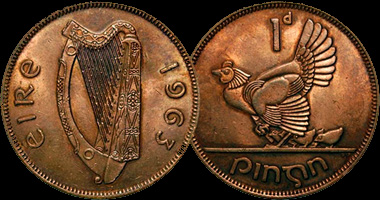
\includegraphics[width=4cm]{coin.jpg}
  \end{center}
We would say \cor{}$p(\mbox{harps})=0.5$\cob.
\end{frame}



\begin{frame}{Probabilities - what do they mean?}
An unknown unfair coin!
  \begin{center}
    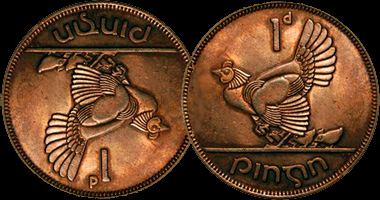
\includegraphics[width=4cm]{coin_2tail.png}\qquad or \qquad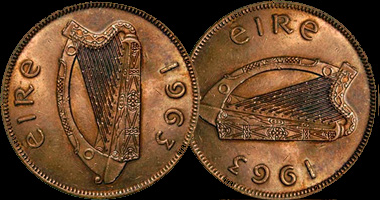
\includegraphics[width=4cm]{coin_2harp.png}
  \end{center}
What if we were told
that the coin was not fair but either both sides are harps or both
sides are heads. Would we then say \cor{}$p(\mbox{harps})=0.5$\cob;
perhaps, but in this case our response to an experiment would be very
different.
\end{frame}



\begin{frame}{Probabilities - what do they mean?}
The usual rain example:
  \begin{center}
    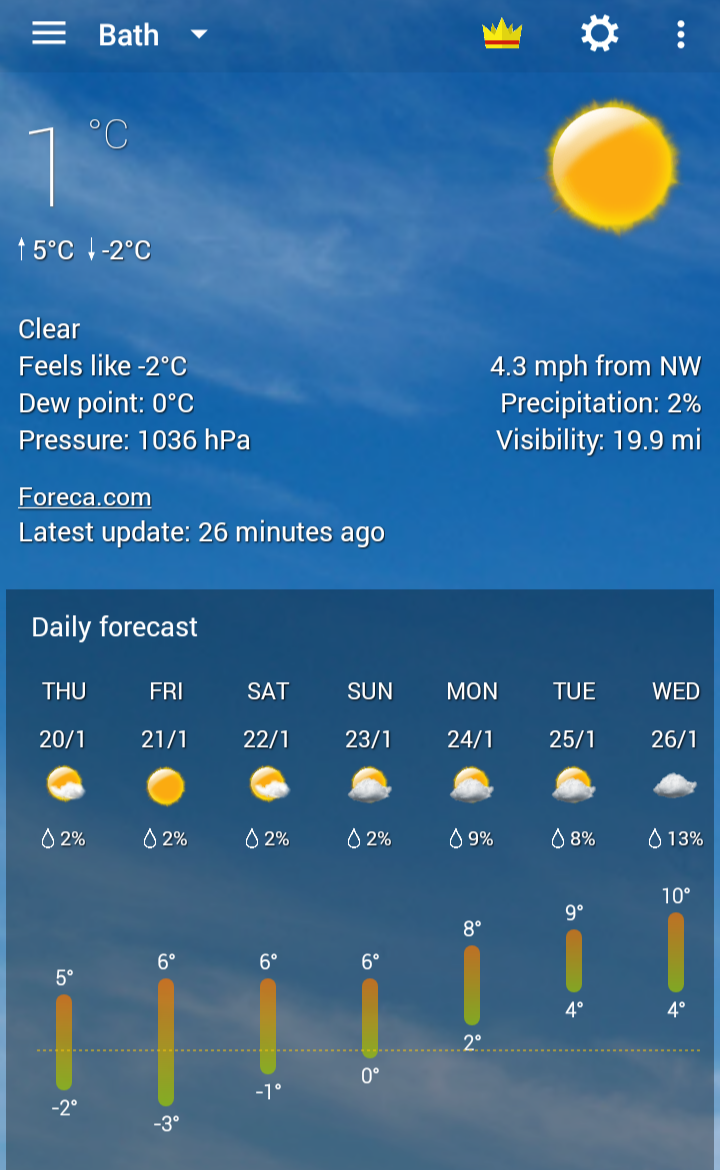
\includegraphics[width=4cm]{rain1.png}
\end{center}
\end{frame}

\begin{frame}{Probabilities - what do they mean?}
The usual rain example:
  \begin{center}
    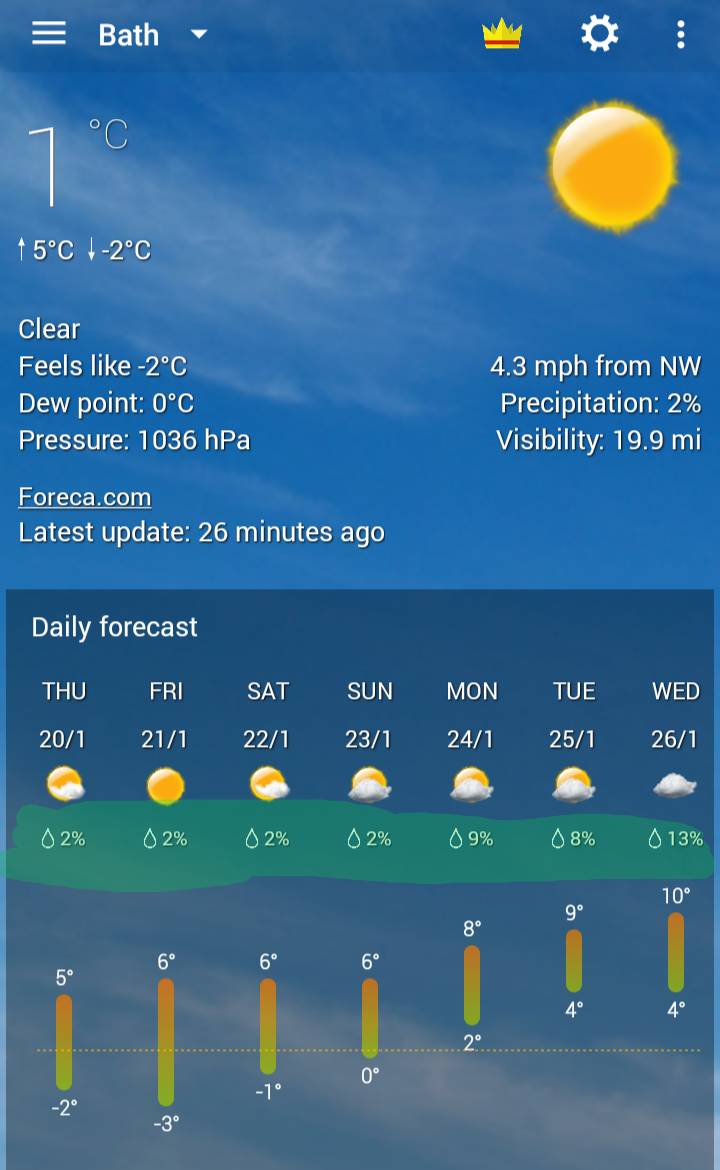
\includegraphics[width=4cm]{rain2.png}
\end{center}
\end{frame}

\begin{frame}{Probabilities - what are they?}
Mathematically
  \begin{quote}
    Probabilities are numerical quantities, defined on a set of
    `outcomes', that are nonnegative, additive over mutually exclusive
    outcomes, and sum to one over all possible mutually exclusive
    outcomes.
  \end{quote}
  \cor
  $$\mbox{outcome}\mapsto p(\mbox{outcome})$$
  \cob
  with some sensible properties.
\end{frame}

\begin{frame}{Probabilities - what are they good for?}
\begin{quote}
In \textbf{Bayesian statistics}, probability is used as the fundamental measure or yardstick of
uncertainty.
\end{quote}
\end{frame}

\begin{frame}{Probabilities - what are they good for?}
\begin{quote}
In \textbf{Bayesian statistics}, probability is used as the fundamental measure or yardstick of
uncertainty.
\end{quote}
\begin{quote}
Within this paradigm, it is equally legitimate to discuss the probability of
`rain tomorrow' or of a Brazilian victory in the soccer World Cup as it is to discuss the
probability that a coin toss will land heads.
\end{quote}
\end{frame}

\begin{frame}{Probabilities - what are they good for?}
\begin{quote}
\textbf{Bayesian methods} enable statements to be made about the
partial knowledge available (based on data) concerning some situation
or `state of nature' - unobservable or as yet unobserved - in a
systematic way, using probability as the yardstick. The guiding
principle is that the state of knowledge about anything unknown is
described by a probability distribution.
\end{quote}
\end{frame}

\begin{frame}{Football example}

  A \textsl{point-spread} is a prediction from a pundit or betting
  firm of a score difference for a football game, the idea being the
  result is equally likely to be higher or lower than the point
  spread. In betting the vig is provided by the point spread with
  payout coming for higher or lower.

\end{frame}


\begin{frame}{Football example 1981 / 1983 / 1984}

\begin{center}
    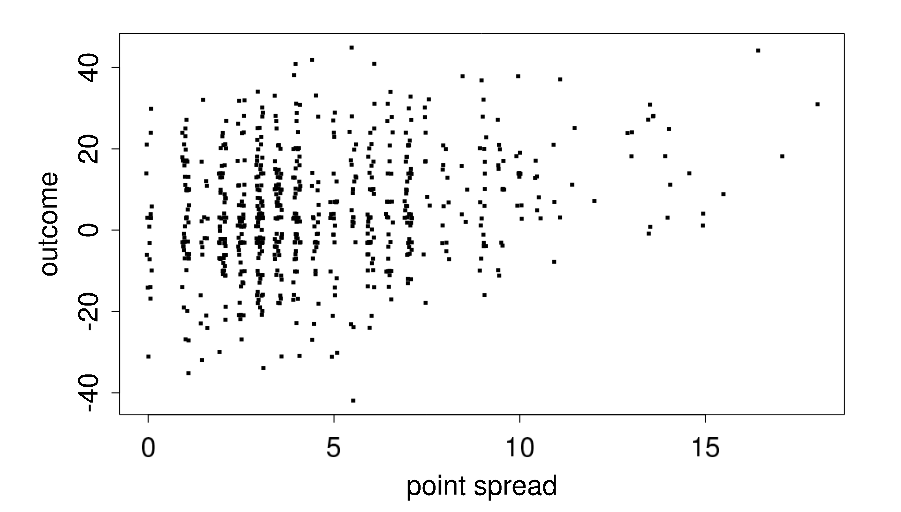
\includegraphics[width=8cm]{football_results.png}
\end{center}

The \coblu{}horizontal axis\cob{} is the point spread, \coblu{}vertical axis\cob{} is actual score for favourite minus underdog; some jitter has been added.
\vfill
\color{gray}figure from the book\cob

\end{frame}

\begin{frame}{Football example - what do we want to know}
  Examples of questions we'd like to ask are
\vskip 0.75cm
  \begin{itemize}
  \item probability of favourite wins \cor{}Pr(favourite wins)\cob
  \item \cor{}Pr(favorite wins $|$ PS is 3.5)\cob
  \item \cor{}Pr(favorite wins by more than the PS)\cob
  \item \cor{}Pr(favorite wins by more than the PS $|$ PS is 3.5)\cob
  \end{itemize}
  \vskip 0.75cm
  and so on; PS is point-spread.
\end{frame}


\begin{frame}{Football example - counting things}
The `intuitive' approach is to count outcomes
\vskip 0.75cm
\begin{itemize}
  \item \cor{}Pr(favourite wins)=410.5/655=0.63\cob
  \item \cor{}Pr(favorite wins $|$ PS is 3.5)=46/59=0.61\cob
  \item \cor{}Pr(favorite wins by more than the PS)=308/655=0.47\cob
  \item \cor{}Pr(favorite wins by more than the PS $|$ PS is 3.5)=32/59=0.54\cob
\end{itemize}
\vskip 0.75cm
where the zero point-spread games are ignored and a draw is a 0.5 win. This all looks sensible and useful.
\end{frame}

\begin{frame}{Football example - intuitive approach stops working}
 
  \begin{itemize}
  \item \cor{}Pr(favourite wins$|$PS is 8.5)=5/5=1\cob
  \item \cor{}Pr(favourite wins$|$PS is 9)=13/20=0.65\cob
  \end{itemize}
\vskip 0.75cm
  This is obviously wrong or mysterious, we could just give up and say the high PS region is undersampled, however, we could make a model, or more correctly, a different model.
\end{frame}


\begin{frame}{Football example 1981 / 1983 / 1984}

\begin{center}
    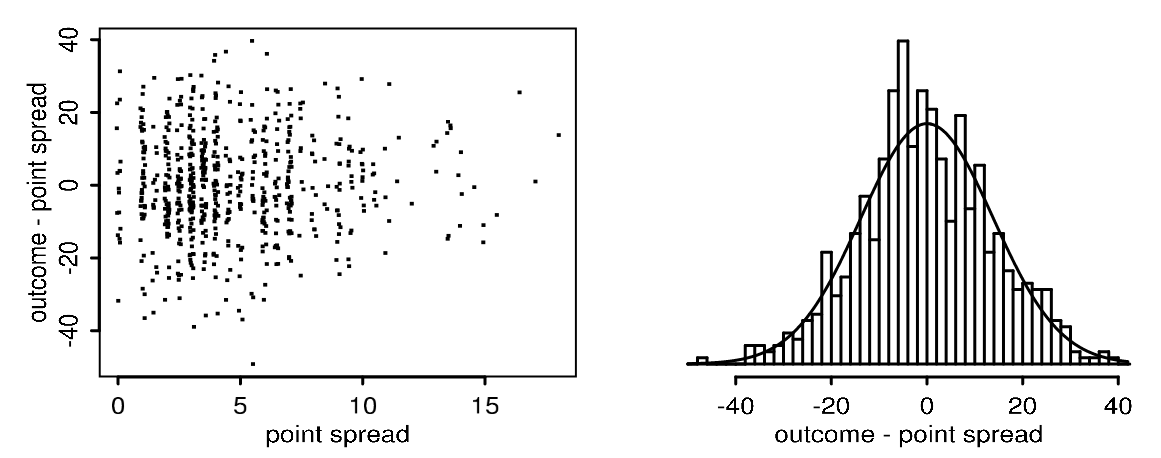
\includegraphics[width=8cm]{football_noise.png}
\end{center}
The black line on the right is \cor{}Normal$(0,14^2)$\cob.
\vfill
\color{gray}figure from the book\cob
\end{frame}


\begin{frame}{Football example - model}

\begin{center}
    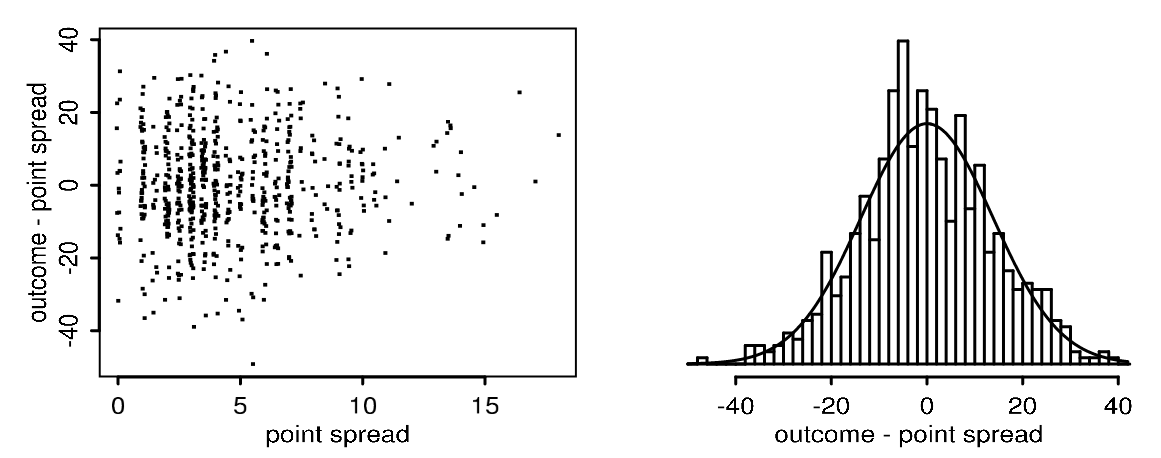
\includegraphics[width=8cm]{football_noise.png}
\end{center}
\cor
\begin{center} score = PS + $\xi$\end{center}
  \cob{}where\cor
  $$\xi\sim \mbox{Normal}(0,14^2)$$
  \cob
  and the basic assumption is that the \cor{}score minus PS\cob{} is independent of  \cor{}PS\cob.
  \vfill
\color{gray}figure from the book\cob
\end{frame}

\begin{frame}{Football example - intuitive approach stops working}
 
  \begin{itemize}
  \item \cor{}Pr(favourite wins$|$PS is 3.5)=0.60\cob
  \item \cor{}Pr(favourite wins$|$PS is 8.5)=0.73\cob
  \item \cor{}Pr(favourite wins$|$PS is 9)=0.74\cob
  \end{itemize}
  \vskip 0.75cm
  which is sensible and maybe even useful, but ignores the
\textbf{errors} in the model: \cor{}score minus PS\cob{} is probably neither
precisely normal nor precisely independent of \cor{}PS\cob{} and it
\textbf{erases} the potential discovery of something special about
games with PS of 8.5.
\end{frame}

\end{document}
